\documentclass{article}

\usepackage[inline]{enumitem}

\usepackage{url}
\usepackage{graphicx}
\usepackage{epsfig}
\graphicspath{ {./figures/} }
\usepackage{amsfonts}% to get the \mathbb alphabet
\usepackage{booktabs}
\usepackage{multirow}


\title{Mining Syndicate: Resisting Mining Centralisation in Bitcoin}
\author{Kulpreet Singh}
\date{\today}

\begin{document}

\maketitle

\begin{abstract}
Large miners have demanded FPPS from their pool operators to eliminate
variance from their earnings. Pool operators have responded and
provided the FPPS payout option. To prevent going bankrupt these pools
have inturn pooled their capital. The providers of capital to the
centralised pool operators has become a potential centralised point of
failure for bitcoin.

The ideal soution is a fully decentralised mining network with all
miners running a bitcoin node. Braidpool is a design striving to
provide such a solution. The problems with braidpool's current design
are that miners don't want to run a bitcoin node and maintain it. It
is also far more challenging to run consensus on a P2P network as well
as a threshold signature scheme on a large network.

We present a solution that hits a middle ground of decentralised
mining pool. The pool is composed of a federation of pool service
providers, called PSPs. Miners interact with any of the PSPs to
receive work and submit their shares. Miners also collect their
payouts from pool service providers. The pool service providers
provide liquidity for miner payouts. In return, the PSPs earn a yield
from their liquidity. Our solution allows anyone to contribute to
running a decentralised pool by joining a federation, providing
liquidity and optionally building block templates.

We show that neither the PSP nor miners can cheat or stop the network
from making progress as long as a $\lfloor (n-1)/3 \rfloor$ PSPs are
honest.

By reducing the threshold cryptography to run only between PSPs and by
removing the friction for miners to run a bitcoin node and build their
own block templates, we allow for the pool to scale to much larger
number of miners. At the same time, our solution enables anyone to
become a pool federation member and provide block templates to miners.
\end{abstract}
   
\section{Solution Overview}

We propose building a federation of Pooling Service Providers, or
PSPs. These PSPs replace pool operators and are completely replacable
from the miner's perspective. As long as a $\lfloor (n-1)/3\rfloor$
PSPs are honest, the miners can keep making progress and withdrawing
their earnings.

A system overview is presented in Figure \ref{fig:system-overview}
that shows that PSPs are arranged in a fully connected point to point
network, miners register with one or more PSPs and that miners
interact with stratum server from any of the PSPs.

\begin{figure}
  \begin{center}
    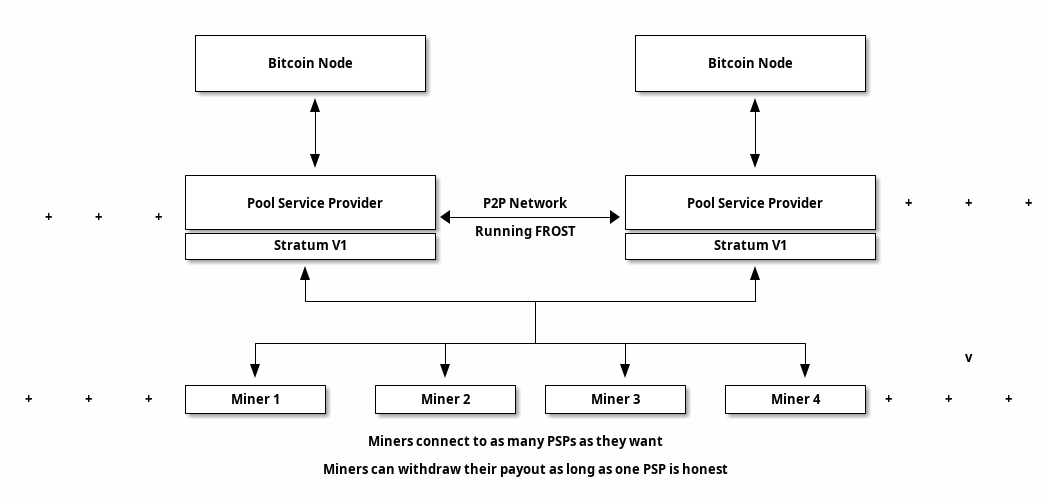
\includegraphics[width=0.75\textwidth]{figures/system-overview}
    \caption{System Overview}\label{fig:system-overview}
  \end{center}
  \label{fig:system-overview}
\end{figure}

The system is composed of the following components that work together:
\begin{enumerate}
\item Threshold Signatures between the PSPs
\item Reliable broadcast between PSPs to provide replicated storage of
  shares
\item Stratum servers run by PSPs
\item Payout mechanism for PSPs to pay miners
\item Liquidity management mechanism for federation members  
\end{enumerate}

We provide an introduction to each of these components and then
present the Bitcoin contracts for the payout and liquidity management
mechanisms.

\subsection{Pool Service Providers}

Anyone can join the PSP network and start contributing towards running
the decentralised pool. As PSPs join the network, they commit funds
that are used to pay the miners. In return for locking their captial,
the PSPs earn a fee for funding the payouts to miners. When PSPs leave
the network, they can withdraw any of their funds that are not
committed to be paid to miners.

It is important to note that a PSP is able to join and leave the
federation without disrupting the working of the pool.

A new member can join the federation by sending a request to an
existing federation member and signing a transaction with two inputs
as show in Figure \ref{fig:funding}. The existing funding members
generate the required threshold signatures to sign the funding
transaction as required by the new member protocol.

\begin{figure}
  \begin{center}
    \includegraphics[width=0.45\textwidth]{figures/funding}
    \caption{New member funding tx}\label{fig:funding}
  \end{center}
  \label{fig:funding}
\end{figure}

The Federation transaction outputs pay out the funders (and the
miners).

\subsection{BFT Consensus and Threshold Signatures for PSPs}

As we saw earlier, the PSPs need to replicate the accounting
information for all miners. This enables the any PSP to step in for a
PSP under a DDoS attack or encountering any other failure.

We will see later, that the PSPs need to run a threshold signature
scheme to provide a key and signature for bitcoin transactions that
result in payouts for miners.

\subsection{Stratum Servers}

All PSPs run a stratum server, and miners can interact with one or
more of these stratum servers at the same time. The shares miners send
to any PSP are replicated to other PSPs - providing an open replicated
pseudonomous database of shares that can be later used to provide
other services for miners. The replication of this data also makes the
mining pool resilient to failures.

\subsection{Payout Mechanism}

How the payouts are claimed by miners needs to meet a few
requirements:

\begin{enumerate}
  \item A miner is unable to cheat other miners of PSPs
  \item A PSP is unable to cheat other PSPs or miners.
  \item A miner can withdraw all their payout at any time, without
    disrupting the operation of the pool.
  \item A PSP can withdraw their non-committed liquidity without
    disrupting the pool's operation.
\end{enumerate}

In the following section, we describe each of these components in
detail and show how the pool is able to provide a decentralised
federation of pool service providers reduces the centralisation
currently seen in bitcoin mining.


\section{Pool Service Providers}

\begin{enumerate}
  \item Run bitcoin nodes and build block templates
  \item Run stratum servers
  \item Miners obtain authentication tokens to use with stratum
\end{enumerate}

\subsection{P2P Network of PSPs}

Gossip based reliable broadcast

HotStuff is used to provide a replicated state machine across PSPs

\subsection{Threshold Signatures}

FROST threshold signatures is used to generate signatures for bitcoin
transactions

\subsection{Federation Membership Management}


Any entity offers BTC liquidity to join the federation

The offered liquidity is managed by the PSP threshold signature.

One a PSP has joined the federation, they need to run an exit
  protocol to leave the federation. As long as a threshold number of
  federation members agree, the PSP can leave the federation.

  
\section{TODO}

- PSP Join protocol - how does the PSP contribute funds to the pool?

- PSP Leave protocol - what happens to funds that the leaving PSP was
contributing? They should be able to leave the network with the left
over funds.

- How is the coinbase reward distributed between PSPs?

- How is the coinbase reward distribution calculated?

- Fidelity bonds by PSP participants? Do they provide any security?


%% \bibliography{tbd} 
%% \bibliographystyle{acm}

\end{document}
